\documentclass[12pt]{report}
\usepackage{polski}
\usepackage[a4paper, margin=2.5cm]{geometry}
\usepackage{graphics}
\usepackage[export]{adjustbox}
\usepackage{float}
\usepackage{amsmath}
\usepackage{xcolor}
\usepackage{multirow}
\usepackage{array}


\title{Analiza wyników pomiarowych z prób spęczania z wykorzystaniem aplikacji komputerowej - praca inżynierska}
\date{12.01.2026}
\author{Szymon Miłkowski}

\begin{document}
	\chapter{Wstęp}
	\section{W pracy}
	\paragraph{}
	Praca obejmuje stworzenie aplikacji komputerowej do graficznej i komputerowej analizy wyników pomiarowych z prób spęczania.
	
	\section{Opis próby spęczania}
	\paragraph{}
	Próba spęczania polega na ściskaniu próbki wzdłuż jednej osi (pionowej) przez maszynę
	badawczą z zadaną prędkością. Podczas próby materiał odkształca się, zmniejszając swoją
	wysokość w kierunku działania siły oraz - zgodnie z zasadą zachowania objętości - zwiększając swoją szerokość w pozostałych kierunkach. Próby mogą być wykonywane w piecu oraz w temperaturze otoczenia - tzn. poza piecem.
	
	\paragraph{}
	Podczas tego procesu, materiał wewnątrz płynie, wypychając materiał na ścianach bocznych na zewnątrz, a materiał przy podstawach trze o górną i dolną ścianę maszyny, co
	hamuje jego przemieszczenie na zewnątrz. Efekt ten powoduje zaokrąglenie powierzchni bocznej próbki.
	
	\paragraph{}
	Wielkości mierzone przez maszynę, zawarte w pliku wyjściowym pomiaru to: czas, obciążenie, przesunięcie oraz zadany sygnał.
	
	\paragraph{}
	Po przeliczeniu wartości sił i przemieszczenia na zależność naprężenia od odkształcenia możliwe jest wyznaczenie granicy plastyczności i wytrzymałości na spęczanie.
	
	\paragraph{}
	Przeprowadzone spęczania w stanie stałociekłym pozwalają również na wyznaczenie wartości lepkości badanego materiału w funkcji prędkości ścinania. (wzory jutro) 
	
	\pagebreak
	\section{Opis maszyny pomiarowej}
	\paragraph{}
	
	\begin{figure}[H]
		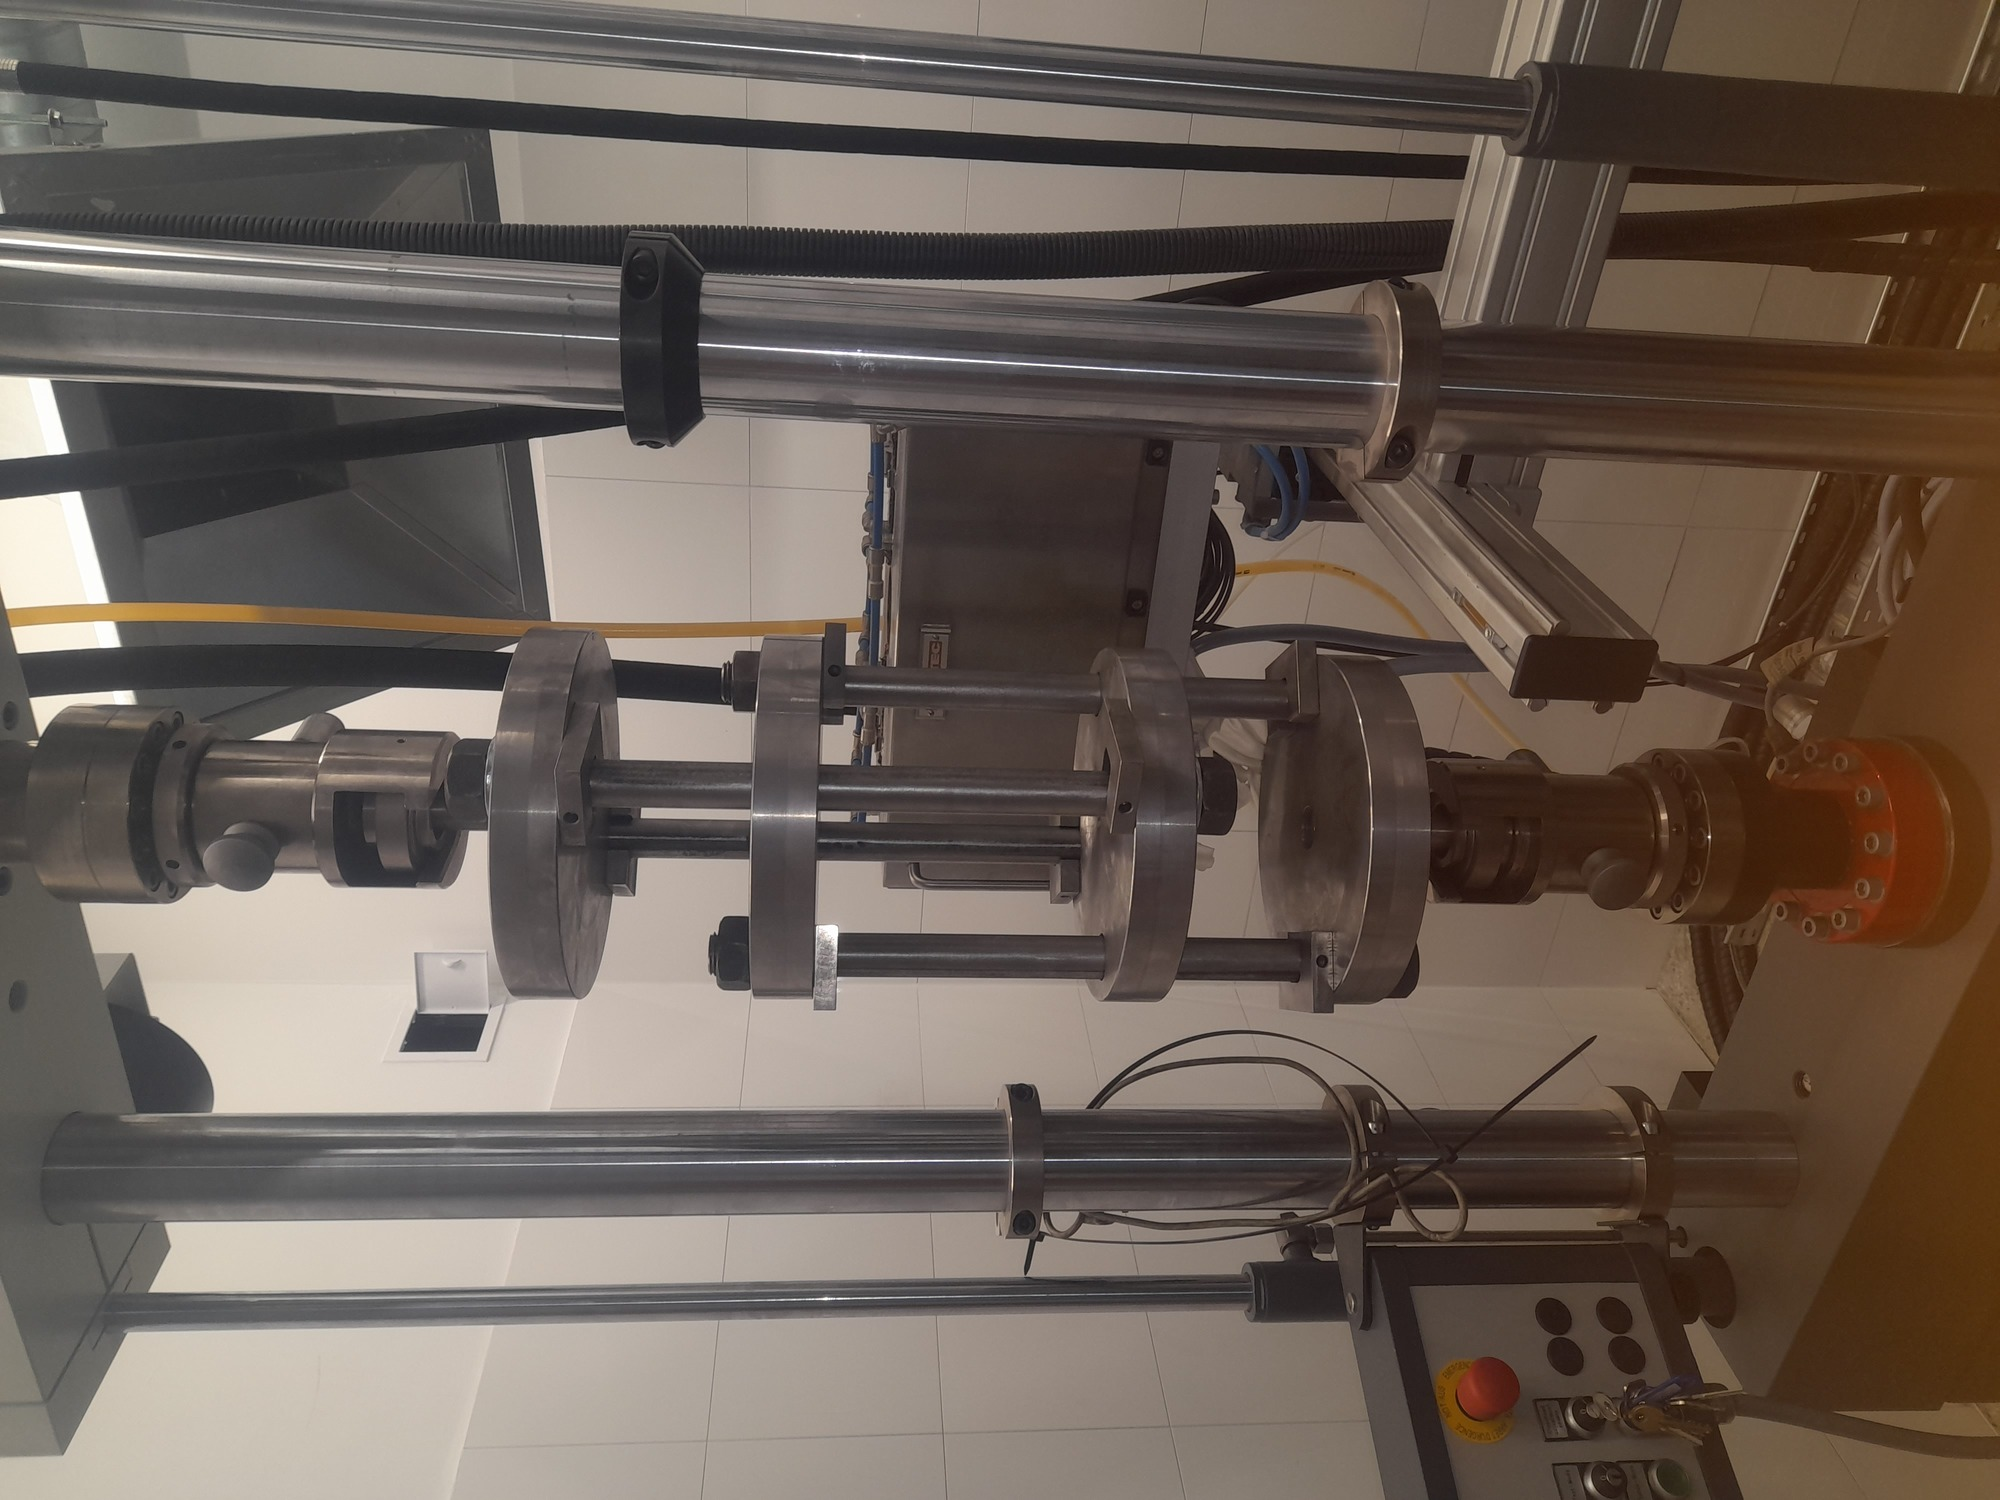
\includegraphics[width=.8\textwidth, angle=-90, center]{images/ZwickHB100a.jpg}
		\caption{Maszyna do przeprowadzania prób spęczania Zwick HB100}
	\end{figure}
	
	\section{Aktualne rozwiązania}
	\subsection{Workshop - moduł data manager}
	\paragraph{}
	Program służy do wyświetlania danych na wykresie. Posiada opcje importu danych z formatu W01, zmiany osi i serii danych oraz eksportu do pliku tekstowego CSV. Program ten jednak jest trudniejszy w obsłudze oraz przydatne funkcjonalności wymagają repetytywnych czynności ze strony użytkownika.
	
	\section{Zawartość pracy}
	\paragraph{}
	Co mieści się w poszczególnych rozdziałach. (wszystko w jednym akapicie, liczby słownie (pierwszy, drugi))
	Ten dokument zawiera opis problemu, cel i założenia, napotkane przeszkody, ogólną strukturę i sposób działania aplikacji oraz niektóre szczegóły implementacji.
	
	
	\chapter{Cel i teza pracy}
	\subsubsection{Cel}
	\paragraph{}
	Celem projektu jest stworzenie kompatybilnego i wydajnego programu, który usprawni
	pracę z wynikami pomiarowymi z prób spęczania. Główny nacisk kładziony jest na maksy-
	malną oszczędność czasu i szybkość w obsłudze dla wprawionego użytkownika, co można
	osiągnąć przez prosty i czytelny interfejs zoptymalizowany pod najczęściej wykonywane
	operacje. Program wykonany w pracy ma na celu obróbkę danych pomiarowych wygenerowanych przez maszynę wytrzymałościową Zwick HB100. Surowe wyniki pomiarów zawierają wartości sił zarejestrowanych dla pozycji siłownika maszyny. W celu wyznaczenia właściwości badanego materiału dane te muszą zostać przeliczone na zależność naprężenia od odkształcenia badanej próbki. Maszyna posiada aplikację do przeglądania wyników prób oraz ich obróbki, niemniej jednak obsługa tego programu jest czasochłonna i nieintuicyjna. Zaplanowane w pracy inżynierskiej oprogramowanie ma na celu istotne skrócenie obróbki danych pomiarowych realizowane przy pomocy interaktywnych wykresów, umożliwiających jednoczesną obserwację kształtu zarejestrowanych zależności.
	
	\paragraph{}
	Dodatkowym celem jest również wysoka kompatybilność programu zarówno z nowymi
	jak i starszymi systemami operacyjnymi oraz wysoka wydajność nawet na starym sprzęcie
	komputerowym.
	
	\subsubsection{Teza}
	Stwierdzono brak powszechnego występowania prostych i darmowych aplikacji umożliwiających obróbkę danych pomiarowych z wykorzystaniem interaktywnych wykresów. W związku z powyższym sformułowano tezę, że analiza wyników pomiarowych jest możliwa dzięki takiemu podejściu, co wykazano w niniejszej pracy.
	
\end{document}